% ─────────────────────────────────────────────────────────────
% CHAPTER 2: HOST ORGANIZATION PROFILE
% ─────────────────────────────────────────────────────────────
\chapter{Host Organization Profile: Digicon Technologies PLC}
\label{ch:organization_profile}

\section{Corporate History and Genesis}
\label{sec:org_history}

\textbf{Digicon Technologies PLC} (formerly Digicon Technologies Ltd.) stands as one of the pioneer and premier Information Technology and Business Process Outsourcing (BPO) conglomerates in Bangladesh. Established in \textbf{2010}, the company was founded with a strategic vision to position Bangladesh as a competitive global destination for IT-enabled services (ITES) and sophisticated enterprise software engineering. Over the past decade and a half, Digicon has undergone exponential institutional expansion, evolving from a boutique contact center into a diversified, multi-vertical technology corporation \citep{digicon2026corp}.

Headquartered strategically at the Rajuk Trade Center in Nikunja-2, Khilkhet, Dhaka, with secondary operational hubs and data facilities situated across Mirpur and Tejgaon, Digicon boasts over 100,000 square feet of state-of-the-art infrastructural space. The organization is a recognized founding and corporate member of the \textbf{Bangladesh Association of Contact Center \& Outsourcing (BACCO)} and maintains strong affiliations with the Bangladesh Computer Samity (BCS) and the Bangladesh Association of Software and Information Services (BASIS) \citep{bacco2024report}.

Throughout its operational history, Digicon has forged strategic partnerships with multinational corporations, domestic telecom giants (including Grameenphone, Robi Axiata, Banglalink, and Teletalk), leading private commercial banks, non-banking financial institutions, multinational pharmaceutical enterprises, and various governmental emergency helplines. The company's consistent adherence to international quality benchmarks is evidenced by its ISO 9001 (Quality Management System) and ISO 27001 (Information Security Management System) certifications, ensuring rigorous data governance and operational integrity across all technical deliveries.

\section{Corporate Vision, Mission, and Core Values}
\label{sec:org_vision_mission}

The operational ethos of Digicon Technologies PLC is anchored upon clear corporate philosophies that drive its engineering methodologies and business customer engagements.

\subsection{Corporate Vision}
\begin{quote}
    \textit{“To be the preeminent technology and outsourcing partner in South Asia, empowering global enterprises through strategic digital transformation, automated operational excellence, and state-of-the-art software solutions.”}
\end{quote}

\subsection{Corporate Mission}
Digicon translates its corporate vision into actionable engineering and service commitments:
\begin{itemize}
    \item \textbf{Technological Innovation:} Continuously engineer robust, scalable, and intuitive software platforms that solve acute enterprise bottlenecks across Customer Relationship Management, messaging, and human capital administration.
    \item \textbf{Operational Excellence:} Maintain uninterrupted 99.98\% uptime across mission-critical customer support services and backend telecommunication gateways.
    \item \textbf{Human Capital Empowerment:} Foster an ecosystem of continuous technical upskilling, mentorship, and professional growth for youth and engineering graduates in Bangladesh.
    \item \textbf{Value Creation:} Deliver measurable Return on Investment (ROI) and cost efficiencies for enterprise partners through agile software automation and intelligent resource routing.
\end{itemize}

\subsection{Core Values}
The corporate and engineering culture at Digicon is underpinned by four core institutional tenets:
\begin{enumerate}
    \item \textbf{Integrity and Confidentiality:} Unwavering adherence to ethical data governance, customer confidentiality, and non-disclosure standards.
    \item \textbf{Agility and Adaptability:} Rapid responsiveness to changing technological landscapes, evolving client specifications, and emergent software design paradigms.
    \item \textbf{Customer Centricity:} Aligning backend architecture and system response times directly with user experience and business customer satisfaction metrics.
    \item \textbf{Collaborative Synergy:} Fostering cross-disciplinary teamwork between software developers, DevOps practitioners, quality assurance testers, and domain business analysts.
\end{enumerate}

\section{Business Domains and Operational Verticals}
\label{sec:org_domains}

Digicon Technologies operates across three primary, mutually reinforcing business pillars: Business Process Outsourcing (BPO) and Contact Center Operations, Software and Technology Solutions, and Professional Training and IT Consultancy.

\subsection{Business Process Outsourcing (BPO) \& Contact Center Solutions}
As a cornerstone of its commercial success, Digicon operates one of the largest contact center infrastructures in Bangladesh:
\begin{itemize}
    \item \textbf{Workforce Scale:} Digicon manages over \textbf{1,500 Full-Time Equivalents (FTEs)} operating in 24/7/365 rotational shifts.
    \item \textbf{Transaction Volume:} The contact center ecosystem processes over \textbf{3 million customer transactions monthly} and manages a daily peak call volume exceeding 1.2 million interactions.
    \item \textbf{Multi-Channel Coverage:} The platform bridges inbound/outbound voice telephony, interactive voice response (IVR), web chat widgets, official social media messaging, and automated ticketing.
    \item \textbf{Global Outreach:} Services are delivered across 14 operational hubs, supporting clients spanning 40+ countries and handling interactions in multiple regional and international languages.
\end{itemize}

\subsection{Software and Technology Solutions Division}
Complementing its service operations, Digicon maintains an extensive internal software engineering wing dedicated to designing custom enterprise software, cloud-native SaaS platforms, and automation tools. The software solutions portfolio includes:

\begin{itemize}
    \item \textbf{Customer Relationship Management (CRM):} A proprietary omnichannel CRM tailored for high-volume contact centers. It provides intelligent ticket routing, real-time agent presence monitoring, automated SLA escalation, and multi-tier customer interaction history.
    \item \textbf{Enterprise SMS \& Telecommunication Gateway:} A high-throughput messaging microservice platform engineered to dispatch transactional notifications, OTP authentication codes, and promotional broadcasts across Bangladesh's telecommunication carriers with sub-second delivery latencies.
    \item \textbf{Human Resource Management System (HRMS):} An integrated enterprise system handling employee attendance, biometric verification, multi-tier leave approval hierarchies, and payroll processing.
    \item \textbf{Enterprise Resource Planning (ERP):} Modular software platforms supporting supply chain management, inventory tracking, field service management, and utility billing for commercial enterprises.
    \item \textbf{Artificial Intelligence \& Conversational Agents:} Natural Language Processing (NLP) chatbots integrated into client web portals to automate tier-1 customer inquiries and deflect repetitive call center volumes.
    \item \textbf{Security Operations Center (SOC) \& Infrastructure Services:} Continuous vulnerability management, network packet inspection, and database security auditing.
\end{itemize}

\subsection{Professional Corporate Training and IT Consultancy}
Digicon provides specialized workforce upskilling programs for corporate entities, preparing technical and non-technical staff in customer interaction standards, cyber hygiene, and modern software tooling. In addition, the firm offers strategic IT consultancy, assisting legacy enterprises in executing seamless migrations to cloud architectures and digital workflows.

\section{Corporate and Engineering Organizational Hierarchy}
\label{sec:org_hierarchy}

The institutional structure of Digicon Technologies PLC is designed to ensure strict executive accountability, fluid cross-departmental communication, and agile technical delivery. Figure~\ref{fig:digicon_org_structure} illustrates the corporate hierarchy and the detailed structure of the Software Engineering Division.

\begin{figure}[htbp]
    \centering
    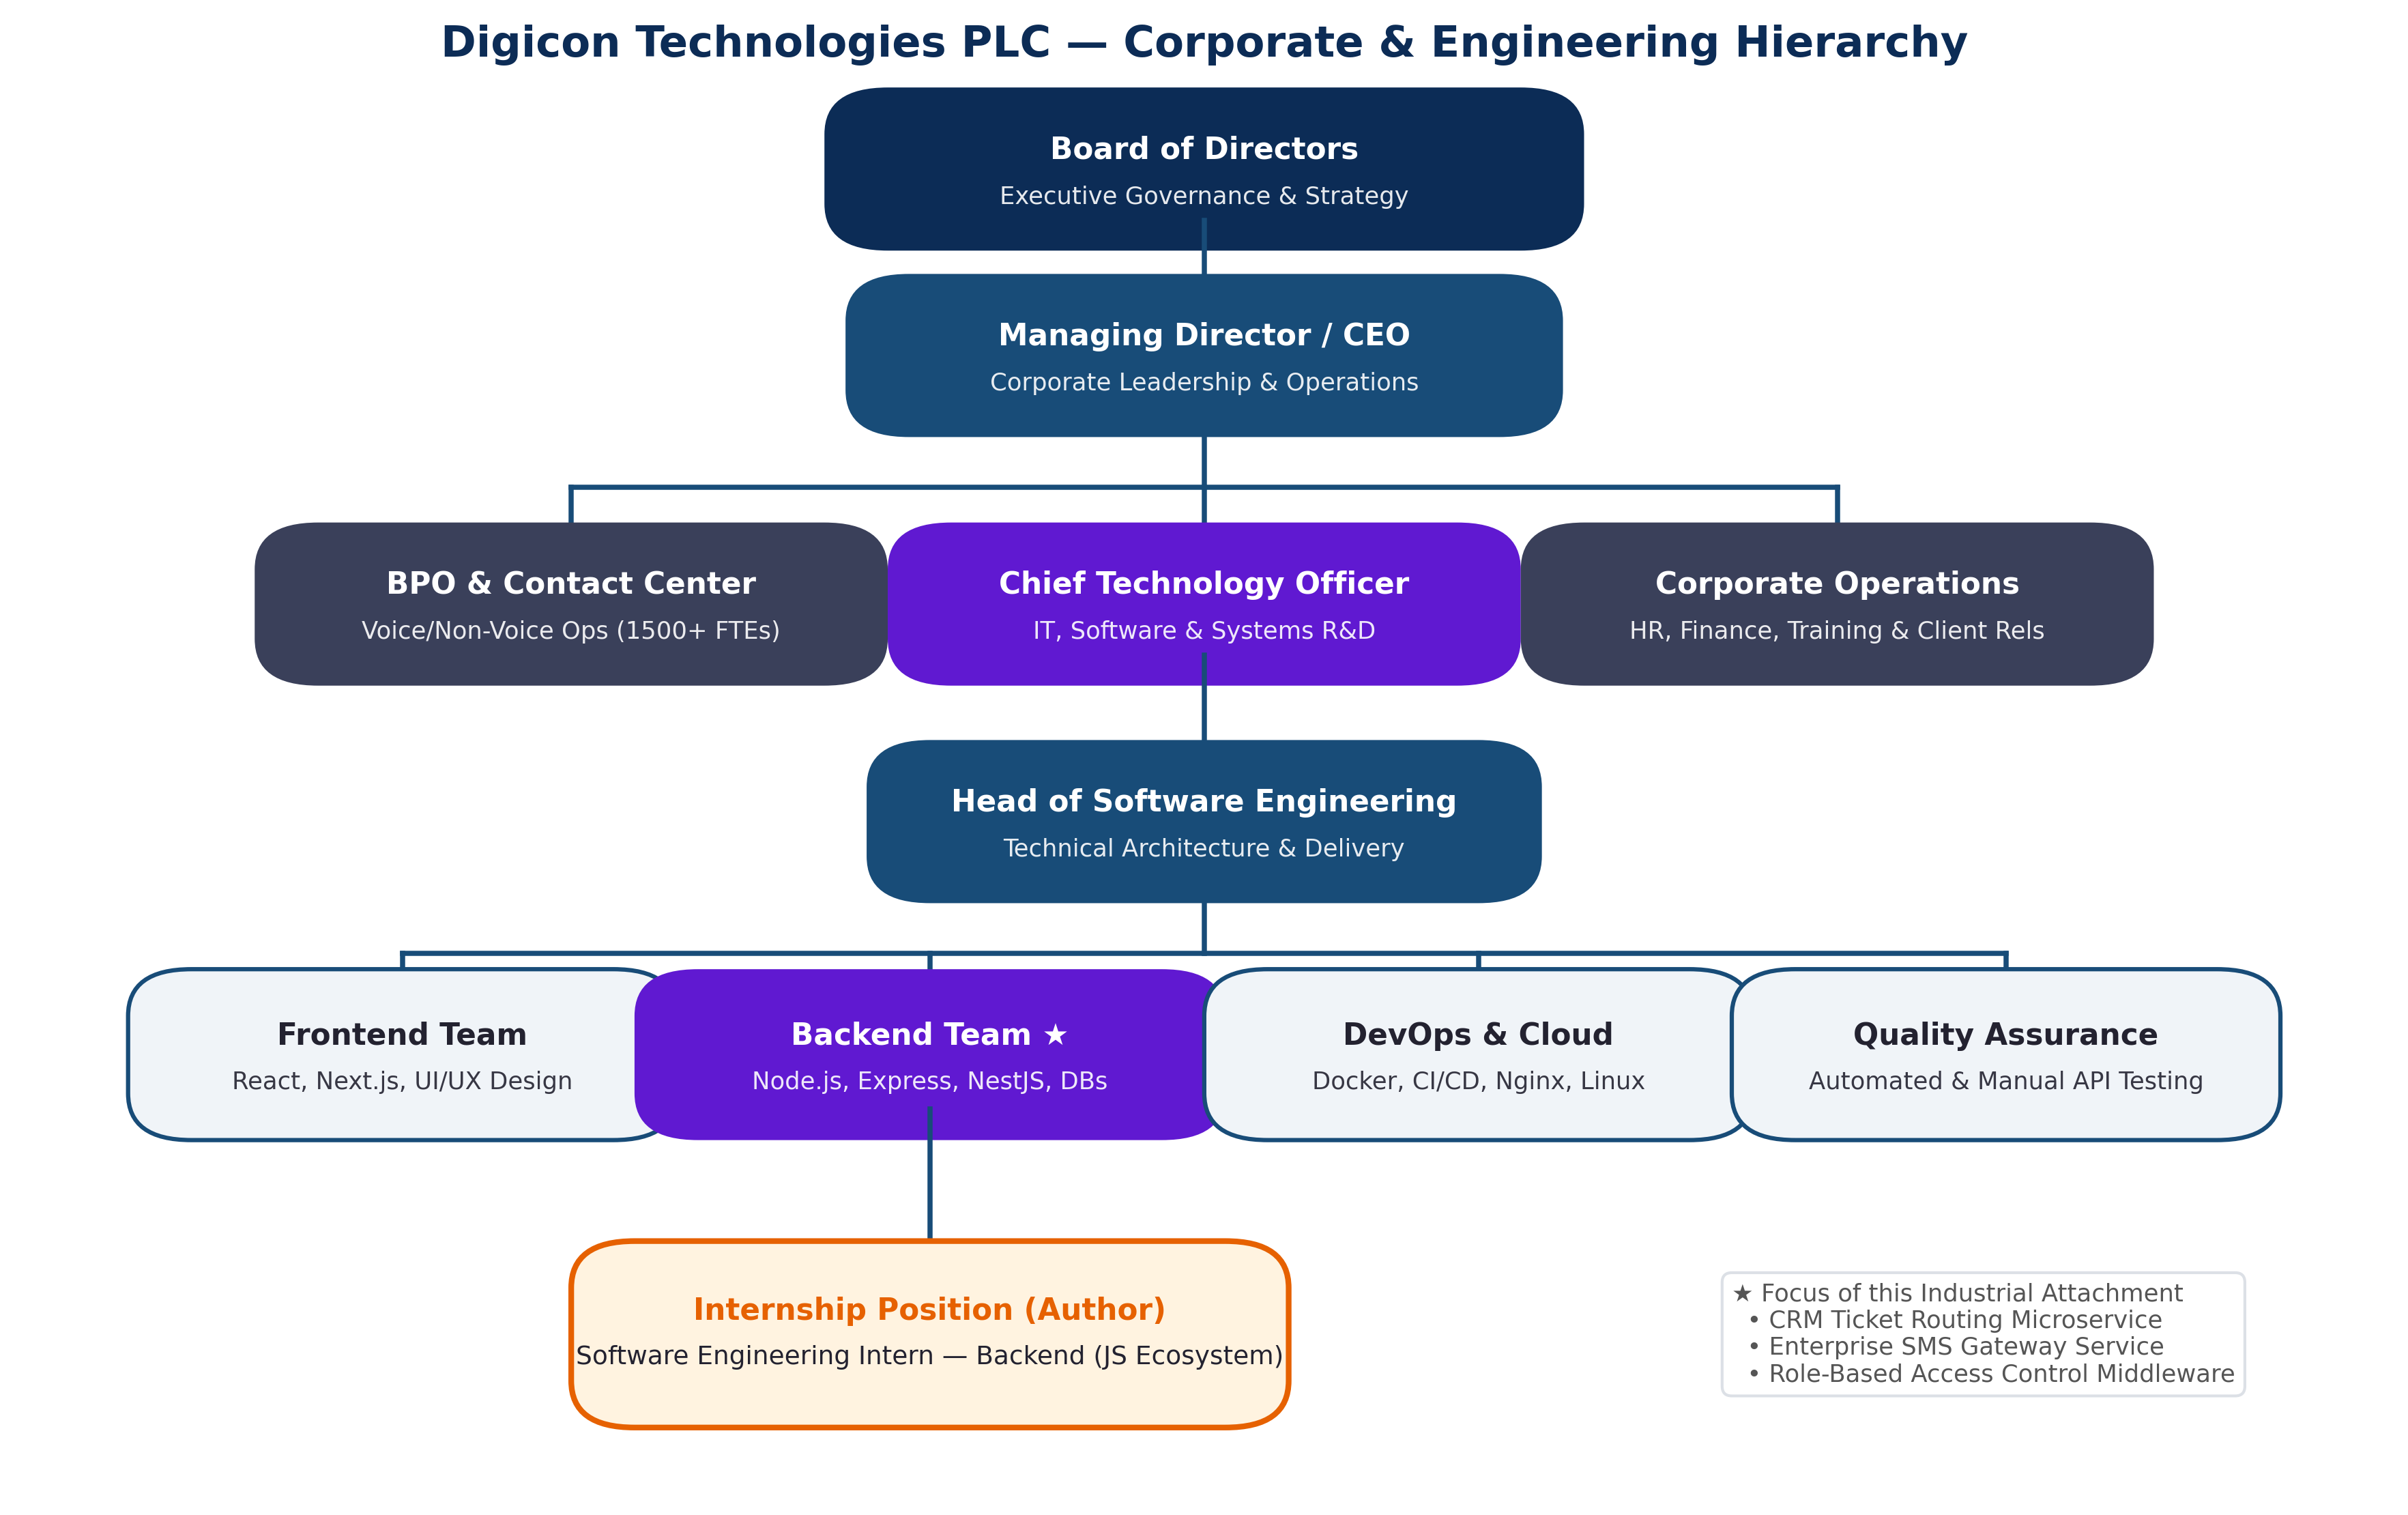
\includegraphics[width=0.95\textwidth]{figures/digicon_org_structure.png}
    \caption{Corporate and Engineering Organizational Hierarchy of Digicon Technologies PLC.}
    \label{fig:digicon_org_structure}
\end{figure}

At the apex of the corporate structure, the \textbf{Board of Directors} exercises strategic governance, capital allocation, and regulatory compliance. The \textbf{Managing Director / Chief Executive Officer (CEO)} oversees overall enterprise performance and commercial growth. Operational execution is partitioned into three key executive wings:
\begin{itemize}
    \item \textbf{BPO Operations Division:} Led by the Head of BPO, managing workforce logistics, contact center quality assurance, and voice operations.
    \item \textbf{Corporate Administration:} Managing human resources, finance, corporate client partnerships, and legal affairs.
    \item \textbf{Technology and Software Division:} Headed by the \textbf{Chief Technology Officer (CTO)}, who steers organizational technology strategy, infrastructure architecture, and R\&D investments.
\end{itemize}

Under the CTO, the \textbf{Head of Software Engineering} directs the day-to-day software development lifecycle. The software engineering division is structured into specialized functional units:
\begin{enumerate}
    \item \textbf{Frontend Engineering Team:} Focuses on responsive user interfaces, design systems, and client-side applications built with React, Next.js, and modern CSS frameworks.
    \item \textbf{Backend Engineering Team (Internship Attachment):} Responsible for system architecture, RESTful and GraphQL API design, database modeling, business logic implementation, caching layers, and external service integrations using Node.js, Express, NestJS, PostgreSQL, MongoDB, and Redis.
    \item \textbf{DevOps \& Cloud Infrastructure Team:} Directs Linux server administration, Docker containerization, CI/CD pipeline automation, Nginx reverse proxy configuration, and cloud network security.
    \item \textbf{Quality Assurance (QA) Team:} Conducts automated regression testing, integration testing, manual acceptance verification, and security vulnerability scanning.
\end{enumerate}

\section{Software Engineering Lifecycle and Methodology}
\label{sec:org_sdlc}

Software engineering at Digicon follows a disciplined, 8-phase development methodology tailored to harmonize enterprise client expectations with rapid technological execution:

\begin{enumerate}
    \item \textbf{Phase 1: Client Idea \& Conceptualization:} Initial stakeholder consultations to identify core operational pain points, high-level business goals, and strategic opportunities.
    \item \textbf{Phase 2: Business Analysis \& Requirement Specification:} Business analysts and software architects decompose client requirements into formal Software Requirement Specifications (SRS), capturing user stories, data schemas, and non-functional constraints.
    \item \textbf{Phase 3: Design Prototype \& Wireframing:} System architects construct architectural blueprints, Entity-Relationship (ER) diagrams, and component interaction models.
    \item \textbf{Phase 4: UI/UX Design:} Product designers develop high-fidelity user interface prototypes and design tokens in Figma.
    \item \textbf{Phase 5: Core Engineering \& Development:} Frontend and backend engineers translate specifications into modular code within two-week Agile/Scrum sprint cycles.
    \item \textbf{Phase 6: Beta Release \& Integration Testing:} Candidate builds are deployed to isolated staging environments for rigorous automated testing, API validation, and user acceptance testing (UAT).
    \item \textbf{Phase 7: Software Launch \& Production Deployment:} Automated CI/CD pipelines deploy verified container images to production clusters behind Nginx load balancers.
    \item \textbf{Phase 8: Continuous Support, Monitoring \& Maintenance:} 24/7 telemetry monitoring via structured logging, performance profiling, and iterative feature enhancements.
\end{enumerate}

\section{Departmental Placement and Intern's Responsibilities}
\label{sec:org_intern_placement}

During the industrial attachment, the author was placed directly within the \textbf{Backend Engineering Team} under the close guidance of the Lead Software Architect. As highlighted in Figure~\ref{fig:digicon_org_structure}, the intern's role was actively integrated into ongoing production sprints rather than confined to passive observation.

The author's primary responsibilities included:
\begin{itemize}
    \item Participating in daily Scrum stand-up meetings, sprint planning, backlog grooming, and technical code reviews.
    \item Architecting and coding modular RESTful controllers and service layers for the internal CRM support ticketing engine.
    \item Building an asynchronous SMS dispatch microservice leveraging Redis BullMQ queues, Token Bucket rate limiting, and webhook cryptographic verification.
    \item Writing comprehensive unit and integration tests using Jest and Supertest to ensure high test coverage and fault tolerance.
    \item Authoring multi-stage Dockerfiles to containerize backend services and optimizing in-memory Redis caching strategies to minimize database latency.
\end{itemize}

This immersion within Digicon's active engineering environment provided the author with firsthand appreciation of how architectural discipline, clean coding standards, and rigorous testing directly impact the reliability of enterprise-scale software systems.
